% !TEX program = lualatex
\documentclass[12pt,a4paper]{article}
\usepackage{fontspec}
\setmonofont{Latin Modern Mono}
\usepackage{xcolor}
\usepackage{listings}
\usepackage{geometry}
\usepackage{fancyhdr}
\usepackage{hyperref}
\usepackage{graphicx}
\geometry{margin=1in}
\usepackage{multicol}

% -------------------------------
% SOLUTION TOGGLE
% -------------------------------
\newif\ifshowsolutions
\showsolutionstrue 
% \showsolutionsfalse

% -------------------------------
% Header and Footer Configuration
% -------------------------------
\pagestyle{fancy}
\fancyhf{}
\lhead{Lab Final}
\rhead{CSE 4308: DBMS Lab}
\cfoot{\thepage}
\setlength{\headwidth}{\textwidth}

% -------------------------------
% Code Listing Style
% -------------------------------
\definecolor{codegreen}{rgb}{0,0.6,0}
\definecolor{codegray}{rgb}{0.5,0.5,0.5}
\definecolor{codepurple}{rgb}{0.58,0,0.82}
\definecolor{backcolour}{rgb}{0.95,0.95,0.92}

\lstdefinestyle{mystyle}{
    backgroundcolor=\color{backcolour},
    commentstyle=\color{codegreen},
    keywordstyle=\color{magenta},
    numberstyle=\tiny\color{codegray},
    stringstyle=\color{codepurple},
    basicstyle=\ttfamily\footnotesize,
    breaklines=true,
    captionpos=b,
    keepspaces=true,
    numbers = none,
    numbersep=5pt,
    tabsize=2,
    frame=single,
    columns=fullflexible,
    showspaces=false,
    showstringspaces=false,
    showtabs=false
}

\lstset{style=mystyle}

% Images: found next to this file (local compile_labs.sh) or via the
% lab folder when compiled from the project root (Overleaf).
\graphicspath{{lab_14_final/}}

\begin{document}

% --------------------------------------------------------------
% TITLE PAGE
% --------------------------------------------------------------
\begin{titlepage}
    \centering
    \vspace*{2\baselineskip}

    \rule{14cm}{2pt}\vspace*{-0.8\baselineskip}\vspace*{1.5pt}
    \rule{14cm}{0.5pt}\vspace{2\baselineskip}

    {\Huge\bfseries\scshape Lab Final\par}
    \vspace{3mm}
    {\Large }
    \vspace{3mm}

    \rule{14cm}{0.5pt}\vspace*{-0.7\baselineskip}\vspace{2.5pt}
    \rule{14cm}{2pt}

    \vspace{2\baselineskip}

    {\Large\bfseries CSE 4308\par}
    \vspace{1\baselineskip}
    {\large DATABASE MANAGEMENT SYSTEMS LAB\par}

    \vfill
    {\normalsize Prepared by:\\ Samnun Azfar, Jr. Lecturer, CSE\\ Samia Nawsheen, Jr. Lecturer, CSE\par}
    {\normalsize Academic Year: AY25-26\par}
\end{titlepage}

\newpage
% ==============================================================
\section{Lab Final}


\begin{enumerate}


% ==============================================================

\item Calculate cost per minute for films, sorted in Descending order.

\ifshowsolutions
\begin{lstlisting}[language=SQL]
SELECT 
    title,
    replacement_cost / length AS cost_per_minute
FROM film
WHERE length > 0
ORDER BY cost_per_minute DESC;
\end{lstlisting}
\fi

% ==============================================================
\item Write a query that returns category name and average film length for categories whose average film length is greater than the overall average film length.

\ifshowsolutions
\begin{lstlisting}[language=SQL]
SELECT cat.name,
       AVG(f.length) AS avg_length
FROM category cat
JOIN film_category fc ON fc.category_id = cat.category_id
JOIN film f ON f.film_id = fc.film_id
GROUP BY cat.name
HAVING AVG(f.length) >
       (SELECT AVG(length) FROM film)
ORDER BY avg_length DESC;
\end{lstlisting}
\fi

% ==============================================================
\item Find customers who have rented the same film more than once. 
Show customer id, full name, film title, and rental count.

\ifshowsolutions
\begin{lstlisting}[language=SQL]
SELECT c.customer_id,
       c.first_name,
       c.last_name,
       f.title,
       COUNT(*) AS rental_count
FROM customer c
JOIN rental r ON r.customer_id = c.customer_id
JOIN inventory i ON i.inventory_id = r.inventory_id
JOIN film f ON f.film_id = i.film_id
GROUP BY c.customer_id, c.first_name, c.last_name, f.title
HAVING COUNT(*) > 1
ORDER BY rental_count DESC, c.customer_id;
\end{lstlisting}
\fi



\item Find actors whose films span all available rating categories. 
Show actor id and full name.

\ifshowsolutions
\begin{lstlisting}[language=SQL]
SELECT a.actor_id,
       a.first_name,
       a.last_name
FROM actor a
JOIN film_actor fa ON fa.actor_id = a.actor_id
JOIN film f ON f.film_id = fa.film_id
GROUP BY a.actor_id, a.first_name, a.last_name
HAVING COUNT(DISTINCT f.rating) =
       (SELECT COUNT(DISTINCT rating) FROM film)
ORDER BY a.actor_id;
\end{lstlisting}
\fi


\item For each city, calculate the total revenue generated by customers from that city sorted in descending order.

\ifshowsolutions
\begin{lstlisting}[language=SQL]
SELECT ci.city, co.country, COALESCE(SUM(p.amount),0) AS revenue
FROM city ci
JOIN address a ON ci.city_id = a.city_id
JOIN customer c ON a.address_id = c.address_id
JOIN payment p ON c.customer_id = p.customer_id
JOIN country co ON ci.country_id = co.country_id
GROUP BY ci.city, co.country
ORDER BY revenue DESC;
\end{lstlisting}
\fi


\item Write an anonymous block that prints the top 5 categories that contain the most films. Print category id, name, and film count using a loop.

\ifshowsolutions
\begin{lstlisting}[language=SQL]
DO $$
DECLARE
    rec RECORD;
    i INT := 0;
BEGIN
    FOR rec IN
        SELECT c.category_id, c.name, COUNT(fc.film_id) AS film_count
        FROM category c
        JOIN film_category fc ON fc.category_id = c.category_id
        GROUP BY c.category_id, c.name
        ORDER BY film_count DESC, c.category_id
    LOOP
        i := i + 1;
        EXIT WHEN i > 5;

        RAISE NOTICE '%) Category %: % (Films=%)',
            i, rec.category_id, rec.name, rec.film_count;
    END LOOP;
END $$;
\end{lstlisting}
\fi


% ==============================================================
\item Write an anonymous block that takes an actor id (e.g., 1) and prints all film titles that the actor appeared in. Print actor name once at the start.

\ifshowsolutions
\begin{lstlisting}[language=SQL]
DO $$
DECLARE
    v_actor_id INT := 1;
    v_first TEXT;
    v_last TEXT;
    rec RECORD;
BEGIN
    SELECT first_name, last_name
    INTO v_first, v_last
    FROM actor
    WHERE actor_id = v_actor_id;

    IF NOT FOUND THEN
        RAISE NOTICE 'Actor % not found', v_actor_id;
        RETURN;
    END IF;

    RAISE NOTICE 'Films for Actor % % (id=%):', v_first, v_last, v_actor_id;

    FOR rec IN
        SELECT f.title
        FROM film f
        JOIN film_actor fa ON fa.film_id = f.film_id
        WHERE fa.actor_id = v_actor_id
        ORDER BY f.title
    LOOP
        RAISE NOTICE ' - %', rec.title;
    END LOOP;
END $$;
\end{lstlisting}
\fi

% \item Write an anonymous block that prints films that have only 3 copies in the inventory. Print film\_id, title, and copy count.

% \ifshowsolutions
% \begin{lstlisting}[language=SQL]
% DO $$
% DECLARE
%     rec RECORD;
% BEGIN
%     FOR rec IN
%         SELECT f.film_id,
%                f.title,
%                COUNT(i.inventory_id) AS copies
%         FROM film f
%         JOIN inventory i ON i.film_id = f.film_id
%         GROUP BY f.film_id, f.title
%         HAVING COUNT(i.inventory_id) = 3
%         ORDER BY f.film_id
%     LOOP
%         RAISE NOTICE 'Film %: % (Copies=%)',
%             rec.film_id, rec.title, rec.copies;
%     END LOOP;
% END $$;
% \end{lstlisting}
% \fi


\item Create a procedure that inserts a payment for that rental using the same customer\_id and staff\_id from \texttt{rental} and uses today's date. 
If \texttt{p\_amount <= 0} or if the rental id does not exist, raise an exception.

\ifshowsolutions
\begin{lstlisting}[language=SQL]
CREATE OR REPLACE PROCEDURE pay_fine(p_rental_id INT, p_amount NUMERIC)
LANGUAGE plpgsql
AS $$
DECLARE
    v_customer_id INT;
    v_staff_id INT;
BEGIN
    IF p_amount <= 0 THEN
        RAISE EXCEPTION 'Amount must be positive';
    END IF;

    SELECT customer_id, staff_id
    INTO v_customer_id, v_staff_id
    FROM rental
    WHERE rental_id = p_rental_id;

    IF NOT FOUND THEN
        RAISE EXCEPTION 'Rental id % not found', p_rental_id;
    END IF;

    INSERT INTO payment(customer_id, staff_id, rental_id, amount, payment_date)
    VALUES (v_customer_id, v_staff_id, p_rental_id, p_amount, NOW());

    RAISE NOTICE 'Payment inserted for rental % (amount=%)', p_rental_id, p_amount;
END;
$$;

-- Invocation (example)
CALL pay_fine(1, 3.50);
\end{lstlisting}
\fi

% ==============================================================
% \item Create a function that returns customers who have rented films from every category.
% Return: customer\_id, full\_name.

% \ifshowsolutions
% \begin{lstlisting}[language=SQL]
% CREATE OR REPLACE FUNCTION customers_who_rented_all_categories()
% RETURNS TABLE (
%     customer_id INT,
%     full_name TEXT
% )
% LANGUAGE plpgsql
% AS $$
% DECLARE
%     v_total_categories INT;
% BEGIN
%     SELECT COUNT(*) INTO v_total_categories FROM category;

%     RETURN QUERY
%     SELECT c.customer_id,
%            (c.first_name || ' ' || c.last_name) AS full_name
%     FROM customer c
%     JOIN rental r ON r.customer_id = c.customer_id
%     JOIN inventory i ON i.inventory_id = r.inventory_id
%     JOIN film_category fc ON fc.film_id = i.film_id
%     GROUP BY c.customer_id, c.first_name, c.last_name
%     HAVING COUNT(DISTINCT fc.category_id) = v_total_categories
%     ORDER BY c.customer_id;
% END;
% $$;

% -- Example:
% SELECT * FROM customers_who_rented_all_categories();
% \end{lstlisting}
% \fi

% ==============================================================
\item Create a function that returns the actor pair (actor1\_id, actor2\_id) that appeared together
in the most films and the film\_count.

\ifshowsolutions
\begin{lstlisting}[language=SQL]
CREATE OR REPLACE FUNCTION most_frequent_actor_pair()
RETURNS TABLE (
    actor1_id SMALLINT,
    actor2_id SMALLINT,
    film_count INT
)
LANGUAGE plpgsql
AS $$
BEGIN
    RETURN QUERY
    SELECT fa1.actor_id,
           fa2.actor_id,
           COUNT(*)::INT
    FROM film_actor fa1
    JOIN film_actor fa2
      ON fa1.film_id = fa2.film_id
     AND fa1.actor_id < fa2.actor_id
    GROUP BY fa1.actor_id, fa2.actor_id
    ORDER BY COUNT(*) DESC, fa1.actor_id, fa2.actor_id
    LIMIT 1;
END;
$$;

-- Example:
SELECT * FROM most_frequent_actor_pair();
\end{lstlisting}
\fi

\item Write a procedure that determines whether a film is above average in rentals by comparing its rental count to the average rental count per film. 

\ifshowsolutions
\begin{lstlisting}[language=SQL]
CREATE OR REPLACE PROCEDURE check_film_popularity_proc(p_film_id INT)
LANGUAGE plpgsql
AS $$
DECLARE
    v_title TEXT;
    v_count INT;
    v_avg NUMERIC;
BEGIN
    -- Get film title
    SELECT title
    INTO v_title
    FROM film
    WHERE film_id = p_film_id;

    IF NOT FOUND THEN
        RAISE NOTICE 'Film id % not found', p_film_id;
        RETURN;
    END IF;

    -- Rental count for this film
    SELECT COUNT(r.rental_id)
    INTO v_count
    FROM inventory i
    JOIN rental r ON r.inventory_id = i.inventory_id
    WHERE i.film_id = p_film_id;

    -- Average rental count per film
    SELECT AVG(cnt)
    INTO v_avg
    FROM (
        SELECT COUNT(r2.rental_id) AS cnt
        FROM inventory i2
        JOIN rental r2 
            ON r2.inventory_id = i2.inventory_id
        GROUP BY i2.film_id
    ) sub;

    -- Compare and print result
    IF v_count > v_avg THEN
        RAISE NOTICE 
        'Film: % | Rentals: % | Avg: % -> ABOVE average',
        v_title, v_count, ROUND(v_avg, 2);
    ELSE
        RAISE NOTICE 
        'Film: % | Rentals: % | Avg: % -> NOT above average',
        v_title, v_count, ROUND(v_avg, 2);
    END IF;
END;
$$;

CALL check_film_popularity_proc(1);
\end{lstlisting}
\fi

\end{enumerate}
\newpage
\section{ER Diagram}
\begin{figure}[h]
        \centering
        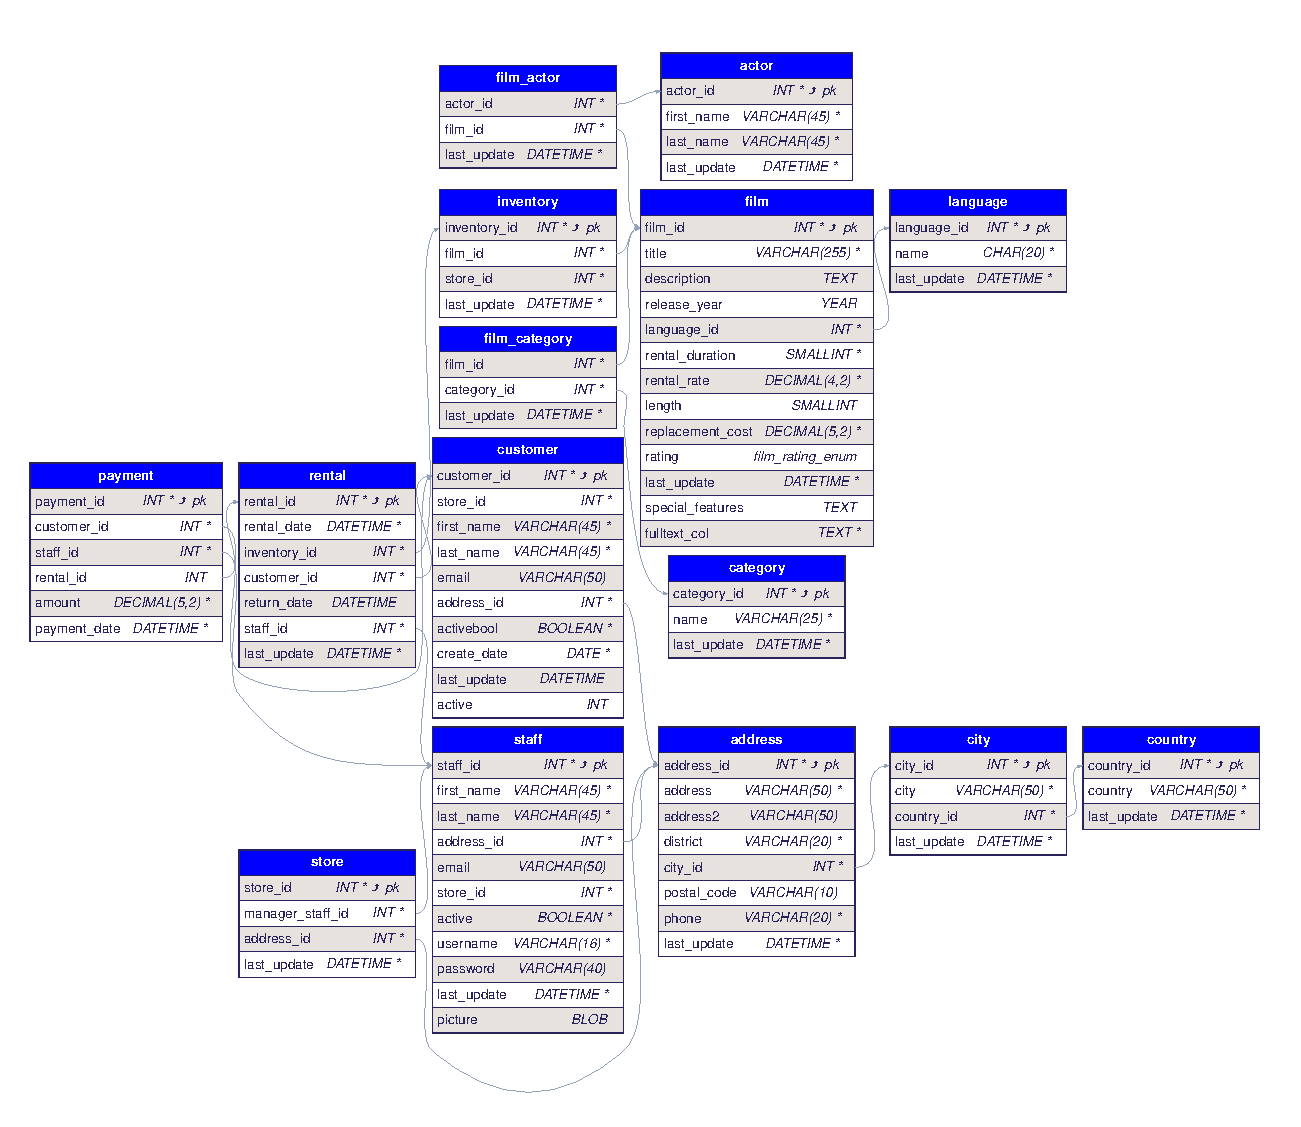
\includegraphics[width=\textheight, height=\textwidth, keepaspectratio, angle=90]{lab_14_schema_cropped.pdf}
\end{figure}

\end{document}